
%------------------------------------------------

\section{Properties of probability}\index{probability!property}
\label{sec:properties-of-probability}

\subsection{Events and sets}\index{probability!event}
\label{subsec:events-and-sets}

The following properties apply to any probability that satisfies the Kolmogorov axioms~(\ref{eq:kolm-1}--\ref{eq:kolm-3}).

A set $A$ of elementary events ${x}_{i}$ can itself be treated as an event.
The occurrence of $A$ is defined as the occurrence of any elementary event ${x}_{i} \in A$.

\begin{equation}
    P(A) = P(\forall {x}_{i} \in A \text{ occurs})
\end{equation}

\subsection{Addition law}\index{probability!addition law}
\label{subsec:addition-law}

Let $A$ and $B$ be non-exclusive sets of elementary events ${x}_{i}$.
The probability of an event belonging to either $A$ or $B$ is given by:

\begin{equation}
    P(A \vee B) = P(A) + P(B) - P(A \wedge B)
\end{equation}

The subtraction term accounts for the overlap between the two sets.

\begin{marginfigure}%[-1.5\baselineskip]
    \begin{tikzpicture}
        \begin{scope}
            \clip \firstcircle;
            \fill[filled] \secondcircle;
        \end{scope}

        \draw[outline] \firstcircle  node[left]  {$A$};
        \draw[outline] \secondcircle node[right] {$B$};

        \node[anchor=south] at (current bounding box.north) {$A \wedge B$};
    \end{tikzpicture}
    \caption{Geometric interpretation of the intersection $A \wedge B$.}
\end{marginfigure}

\subsection{Conditional probability and independence}\index{conditional probability}\index{independence}
\label{subsec:conditional-probability-and-independence}

The probability that an elementary event ${x}_{i}$, known to belong to the set $B$, is also a member of the set $A$ is given by:

\begin{equation}\label{eq:conditional-joint}
    P(A \wedge B) = P(A \mid B) \cdot P(B) = P(B \mid A) \cdot P(A)
\end{equation}

Therefore,

\begin{equation}
    P(A \mid B) = \frac{P(A \wedge B)}{P(B)}
\end{equation}

The sets $A$ and $B$ are independent if:

\begin{equation}
    P(A \mid B) = P(A)
\end{equation}

which means that the previous occurrence of $B$ is irrelevant to the occurrence of $A$.

If $A$ is independent of $B$, the probability of the simultaneous occurrence of $A$ and $B$ is the product of their probabilities:

\begin{equation}
    P(A \wedge B) = P(A) \cdot P(B)
\end{equation}

\subsection{Law of total probability}\index{law of total probability}
\label{subsec:law-of-total-probability}

Consider $N$ events corresponding to the sets ${E}_{1}, {E}_{2}, \cdots, {E}_{N}$, which are subsets of another set $E$ included in the sample space $\Omega$.

Assume that the sets ${E}_{i}$ form a partition of $E$, \ie

\begin{marginfigure}
    \centering
    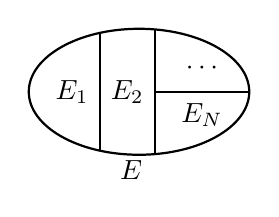
\begin{tikzpicture}

        % Outer set E
        \draw[thick] (0,0) ellipse (1.4 and 0.8);
        \node at (-0.1,-1) {$E$};

        % Partition inside E
        \draw[thick] (-0.5,-0.75) -- (-0.5,0.75);
        \draw[thick] ( 0.2,-0.79) -- ( 0.2,0.79);
        \draw[thick] ( 0.2,    0) -- ( 1.4,   0);

        % Labels
        \node at (-0.85,   0) {${E}_{1}$};
        \node at (-0.15,   0) {${E}_{2}$};
        \node at (  0.8, 0.3) {$\cdots$};
        \node at (  0.8,-0.3) {${E}_{N}$};

    \end{tikzpicture}
    \caption{Partition of the event $E$ into disjoint subsets ${E}_{i}$.}
\end{marginfigure}

\begin{align}
    & {E}_{i} \wedge {E}_{j} = \emptyset, \quad \forall i \neq j, \\
    & \bigvee_{i=1}^{N} {E}_{i} = E.
\end{align}

The probability of the set $E$ is then given by:

\begin{equation}
    P(E) = \sum_{i=1}^{N} P({E}_{i}).
\end{equation}

Now let us choose a disjoint partition ${A}_{1}, {A}_{2}, \cdots, {A}_{N}$ of the sample space $\Omega$, such that:

\begin{marginfigure}
    \centering
    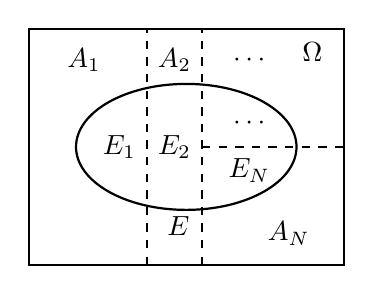
\begin{tikzpicture}

        % Sample space Omega
        \draw[thick] (-2,-1.5) rectangle (2,1.5);
        \node at (1.6,1.2) {$\Omega$};

        % Partition A_i
        \draw[thick, dashed] (-0.5,-1.5) -- (-0.5,1.5);
        \draw[thick, dashed] ( 0.2,-1.5) -- ( 0.2,1.5);
        \draw[thick, dashed] ( 0.2,   0) -- (   2,  0);

        \node at ( -1.3, 1.1) {${A}_{1}$};
        \node at (-0.15, 1.1) {${A}_{2}$};
        \node at (  0.8, 1.1) {$\cdots$};
        \node at (  1.3,-1.1) {${A}_{N}$};

        % Event E
        \draw[thick] (0,0) ellipse (1.4 and 0.8);
        \node at (-0.1,-1) {$E$};

        % Intersection labels
        \node at (-0.85,   0) {${E}_{1}$};
        \node at (-0.15,   0) {${E}_{2}$};
        \node at (  0.8, 0.3) {$\cdots$};
        \node at (  0.8,-0.3) {${E}_{N}$};

    \end{tikzpicture}
    \caption{Partition of the sample space $\Omega$ into ${A}_{i}$ and induced subsets ${E}_{i} = E \wedge {A}_{i}$.}
\end{marginfigure}

\begin{align}
    & \bigvee_{i=1}^{N} {A}_{i} = \Omega, \\
    & {A}_{i} \wedge {A}_{j} = \emptyset, \quad \forall i \neq j, \\
    & \sum_{i=1}^{N} P({A}_{i}) = 1.
\end{align}

Assume further that:

\begin{equation}
    {E}_{i} = E \wedge {A}_{i}.
\end{equation}

We then have:

\begin{equation}
    P({E}_{i}) = P(E \wedge {A}_{i}) = P(E \mid {A}_{i}) \cdot P({A}_{i}).
\end{equation}

Therefore,

\begin{equation}
    P(E) = \sum_{i=1}^{N} P(E \mid {A}_{i}) \cdot P({A}_{i}).
\end{equation}

This result is known as the \mono{``law of total probability''}\index{law of total probability}.

It can be interpreted as a \mono{weighted average}\index{weighted average} of the probabilities $P({A}_{i})$, where the weights ${w}_{i}$ are given by the conditional probabilities $P(E \mid {A}_{i})$.

\subsection{Bayes' theorem for discrete events}\index{Bayes' theorem}
\label{subsec:bayes--theorem-for-discrete-events}

Recall the law of conditional probability for two sets $A$ and $B$, given in Eq.~\eqref{eq:conditional-joint}:

\begin{equation}
    P(A \wedge B) = P(B \mid A) \cdot P(A) = P(A \mid B) \cdot P(B)
\end{equation}

Therefore,

\begin{equation}\label{eq:bayes--discrete}
    P(A \mid B) = \frac{P(B \mid A) \cdot P(A)}{P(B)}
\end{equation}

\begin{figure*}[h]
    \begin{tikzpicture}

        % Sample space Omega
        \draw[thick] (-2,-1.5) rectangle (2,1.5);
        \node at (1.6,1.2) {$\Omega$};

        % Intersection A \wedge B
        \begin{scope}
            \clip (-0.5,0) ellipse (0.8 and 1.4);
            \fill[purple!40] (0.5,0) ellipse (1.4 and 0.6);
        \end{scope}

        \node at (-0.3,0) {$A \wedge B$};

        % Event A (vertical ellipse)
        \draw[thick, blue] (-0.5,0) ellipse (0.8 and 1.4);
        \node[blue] at (-0.5,1) {$A$};

        % Event B (horizontal ellipse)
        \draw[thick, red]  (0.5,0) ellipse (1.4 and 0.6);
        \node[red] at (1.5,0) {$B$};

        % Probability annotations
        \node at (5,1)
        {$P(A)=\dfrac{\qquad \qquad \qquad \qquad}{\qquad \qquad \qquad \qquad}$};
        \draw[thick, blue] (5.65,  1.9) ellipse (0.4 and 0.7);
        \draw[thick]       (5.65-1,0.2-0.75) rectangle (5.65+1,0.2+0.75);

        \node at (10,1)
        {$P(B)=\dfrac{\qquad \qquad \qquad \qquad}{\qquad \qquad \qquad \qquad}$};
        \draw[thick, red]  (10.65,  1.5) ellipse (0.7 and 0.3);
        \draw[thick]       (10.65-1,0.2-0.75) rectangle (10.65+1,0.2+0.75);

        \node at (5,-1.6)
        {$P(A \mid B)=\dfrac{\qquad \qquad \qquad}{\qquad \qquad \qquad}$};
        \begin{scope}
            \clip            (5.85+0.15-0.25,-1.1) ellipse (0.4 and 0.7);
            \fill[purple!40] (5.85+0.15+0.25,-1.1) ellipse (0.7 and 0.3);
        \end{scope}
        \draw[thick, red]    (5.85,          -2.0) ellipse (0.7 and 0.3);

        \node at (10,-1.6)
        {$P(B \mid A)=\dfrac{\qquad \qquad \qquad}{\qquad \qquad \qquad}$};
        \begin{scope}
            \clip            (10.85+0.15-0.25,-1.1) ellipse (0.4 and 0.7);
            \fill[purple!40] (10.85+0.15+0.25,-1.1) ellipse (0.7 and 0.3);
        \end{scope}
        \draw[thick, blue]   (10.85,         -2.35) ellipse (0.4 and 0.7);

        \node at (5,-3.8)
        {$P(A \mid B)\cdot P(B)
            =\dfrac{\qquad \qquad \qquad}{\qquad \qquad \qquad}
                \cdot \dfrac{\qquad \qquad \qquad \qquad}{\qquad \qquad \qquad \qquad}
            =\dfrac{\qquad \qquad \qquad \qquad}{\qquad \qquad \qquad \qquad}
            = P(A \wedge B)$};
            \begin{scope}
                \clip            (2.2+0.15-0.25,-3.3) ellipse (0.4 and 0.7);
                \fill[purple!40] (2.2+0.15+0.25,-3.3) ellipse (0.7 and 0.3);
            \end{scope}
            \draw[thick, red]    (2.2,          -4.2) ellipse (0.7 and 0.3);
            \draw[thick, red]    (5.0,          -3.3) ellipse (0.7 and 0.3);
            \draw[thick]         (5.0-1,        -4.6-0.75) rectangle (5.0+1,-4.6+0.75);
            \begin{scope}
                \clip            (8.4+0.15-0.25,-3.3) ellipse (0.4 and 0.7);
                \fill[purple!40] (8.4+0.15+0.25,-3.3) ellipse (0.7 and 0.3);
            \end{scope}
            \draw[thick]         (8.4-1,        -4.6-0.75) rectangle (8.4+1,-4.6+0.75);

        \node at (5,-7.3)
        {$P(B \mid A)\cdot P(A)
            =\dfrac{\qquad \qquad \qquad}{\qquad \qquad \qquad}
            \cdot \dfrac{\qquad \qquad \qquad \qquad}{\qquad \qquad \qquad \qquad}
            =\dfrac{\qquad \qquad \qquad \qquad}{\qquad \qquad \qquad \qquad}
            = P(A \wedge B)$};
        \begin{scope}
            \clip            (2.2+0.15-0.25,-6.8 ) ellipse (0.4 and 0.7);
            \fill[purple!40] (2.2+0.15+0.25,-6.8 ) ellipse (0.7 and 0.3);
        \end{scope}
        \draw[thick, blue]   (2.2,          -8.05) ellipse (0.4 and 0.7);
        \draw[thick, blue]   (5.0,          -6.4 ) ellipse (0.4 and 0.7);
        \draw[thick]         (5.0-1,        -8.1-0.75) rectangle (5.0+1,-8.1+0.75);
        \begin{scope}
            \clip            (8.4+0.15-0.25,-6.8 ) ellipse (0.4 and 0.7);
            \fill[purple!40] (8.4+0.15+0.25,-6.8 ) ellipse (0.7 and 0.3);
        \end{scope}
        \draw[thick]         (8.4-1,        -8.1-0.75) rectangle (8.4+1,-8.1+0.75);

    \end{tikzpicture}
    \caption{Geometric interpretation of Bayes' theorem.
        Probabilities are represented as ratios of areas within the sample space $\Omega$.}
    \label{fig:bayes-geometry}
\end{figure*}

More generally, let ${A}_{1}, {A}_{2}, \cdots, {A}_{N}$ be \mono{exclusive} and \mono{exhaustive} sets, and let $B$ be any event:

\begin{equation}\label{eq:bayes--discrete-general}
    P({A}_{i} \mid B)
    = \frac{P(B \mid {A}_{i}) \cdot P({A}_{i})}
    {\sum_{i=1}^{N} P(B \mid {A}_{i}) \cdot P({A}_{i})}
\end{equation}

\begin{itemize}
    \item $P({A}_{i})$ is the \mono{``prior probability''}\index{prior probability} of ${A}_{i}$,
    \ie the probability of the set ${A}_{i}$ before the knowledge that event $B$ has occurred.
    \item $P({A}_{i} \mid B)$ is the \mono{``posterior probability''}\index{posterior probability} of ${A}_{i}$,
    \ie the probability of the set ${A}_{i}$ after having collected the information that event $B$ has occurred.
\end{itemize}

\newthought{Example}: measuring protons with particle detectors (Figure~\ref{fig:Bayes__theorem_proton}):

\begin{itemize}
	\item $P(B) = P(+ \wedge p) + P(+ \wedge n) = $ probability of any particle giving a triggered event.
	\item $P(A) = P(+ \wedge p) + P(0 \wedge p) = $ probability of a proton hitting the detector.
	\item $P(B \mid A) = \frac{P(+ \wedge p)}{P(+ \wedge p) + P(0 \wedge p)} = $ probability of a proton giving a triggered event.
	\item $P(A \mid B) = \frac{P(+ \wedge p)}{P(+ \wedge p) + P(+ \wedge n)} = $ probability of a triggered event to be induced by a proton.
\end{itemize}

\begin{figure}
	\includegraphics{probability/Bayes__theorem.pdf}
	\caption[Venn diagram of Bayes' theorem.][6pt]{Venn diagram of Bayes' theorem.}
	\label{fig:Bayes__theorem_proton}
\end{figure}

\subsection{Bayes' theorem for hypotheses testing and parameter estimation}\index{hypothesis test}
\label{subsec:bayes__hypo}

\newthought{Assume} $H_{0}$, $H_{1}$ are a complete set of hypotheses, i.e. a complete set os physics models describing a given physical phenomenon.

For example:

\begin{itemize}
	\item $H_{0} = $ background-only hypothesis\index{hypothesis!background-only} = The known physics processors are enough to explain the data.
	\item $H_{1} = $ signal + background hypothesis\index{hypothesis!signal + background} = There is an additional component due to new physics and that we know how to model.
\end{itemize}

$H_{0}$ and $H_{1}$ will depend on some parameters, which can differ between the two hypotheses, but that we will indicate generally as $\vec{\theta} \in \Omega $.

Let's indicate the data with $\vec{x}$.

\paragraph{Parameter estimation}\index{parameter estimation}

\begin{equation}\label{eq:para_esti}
	P( \vec{\theta} \mid \vec{x} )
	= \frac{P( \vec{x} \mid \vec{\theta} ) \pi(\vec{\theta})}
		{\int_{\Omega} {P( \vec{x} \mid \vec{\theta} ) \pi(\vec{\theta})} \,\mathrm{d}\vec{\theta}}
	= \frac{P( \vec{x} \mid \vec{\theta} ) \pi(\vec{\theta})}
		{P( \vec{x})}
\end{equation}

\begin{itemize}
	\item $P( \vec{\theta} \mid \vec{x} ) = $ posterior probability\index{posterior probability} for parameters $\vec{\theta}$ gives the data $\vec{x}$ and the model $H_{0}$ or $H_{1}$.
		\marginnote{This is valid both for $H_{0}$ and $H_{1}$.}
	\item $P( \vec{x} \mid \vec{\theta} ) = $ probability of obtaining exactly the data $\vec{x}$ gives each possible values of the parameters $\vec{\theta}$.
	\item $\pi(\vec{\theta}) = $ prior probability\index{prior probability} of parameter $\vec{\theta}$ under the assumption of $H_{0}$ or $H_{1}$.
	\item $P(\vec{x}) = $ probability of getting data $\vec{x}$ given any possible value of $\vec{\theta}$ assuming model $H_{0}$ or $H_{1}$.
		\marginnote{In the end, it is a normalization factor.}
\end{itemize}

\newthought{Considering both hypotheses} $H_{0}$ and $H_{1}$:

\begin{equation}
	P( \vec{\theta}, H_{0} \mid \vec{x} )
	= \frac{P( \vec{x} \mid H_{0}(\vec{\theta}) ) \pi( \vec{\theta}, H_{0} )}
		{\sum_{i}{\int_{\Omega} {P( \vec{x} \mid \vec{\theta}_{i}, H_{i} ) \pi( \vec{\theta}_{i}, H_{i} ) \pi(H_{i})} \,\mathrm{d}\vec{\theta}}}
\end{equation} \marginnote[-6pt]{denominator $\to$ \mono{constant}}

\paragraph{Hypothesis testing}\index{hypothesis test}
\begin{equation}\label{eq:hypo_test}
	P(H_{i} \mid \vec{x})
	= \frac{P(\vec{x} \mid H_{i}) \pi(H_{i})}
		{\sum_{i}{P(\vec{x} \mid H_{i}) \pi(H_{i})}}
\end{equation}

\begin{itemize}
	\item $P(H_{i} \mid \vec{x}) = $ posterior probability\index{posterior probability} for hypothesis $H_{i}$ after measuring the data.
	\item $\pi(H_{i}) = $ prior probability\index{prior probability} for hypothesis $H_{i}$.
		\marginnote{This is the \mono{subjective} part of the method.}
	\item $P(\vec{x} \mid H_{i}) = \int_{\Omega} {P( \vec{x} \mid \vec{\theta}, H_{i} ) \pi(\vec{\theta})} \,\mathrm{d}\vec{\theta} = $ probability of obtaining data $\vec{x}$ gives each possible values of the parameters $\vec{\theta}$ assuming model $H_{i}$.
	\item $\sum_{i}{P(\vec{x} \mid H_{i}) \pi(H_{i})} = $ normalization factor.
\end{itemize}

\newthought{Example}: religious belief.
